\documentclass[tikz,border=8pt]{standalone}
\usepackage[T1]{fontenc}
\usepackage[scaled=0.92]{sourcesanspro}
\renewcommand{\familydefault}{\sfdefault}
\usetikzlibrary{arrows.meta,positioning,calc,backgrounds,shapes.geometric,shapes.arrows}
\begin{document}
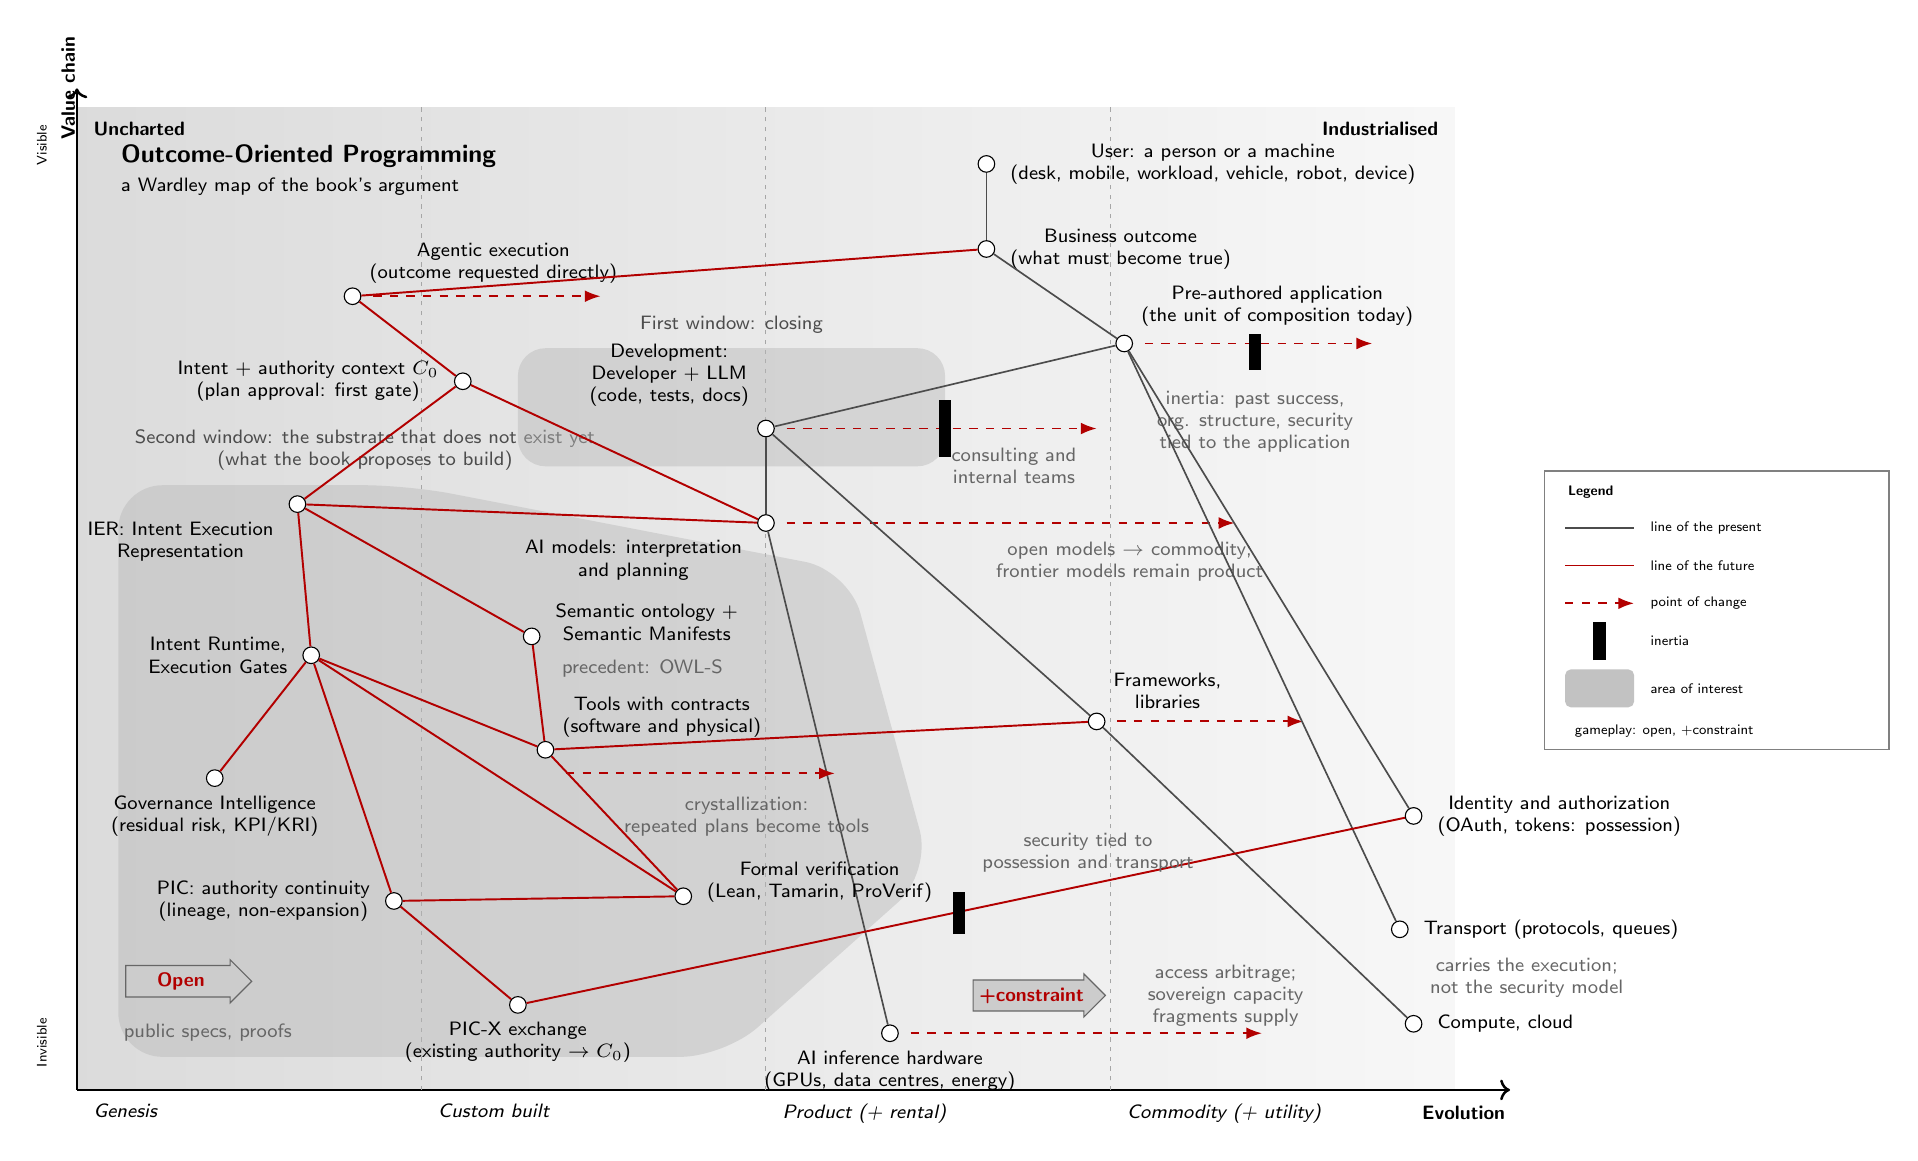
\begin{tikzpicture}[x=1.75cm,y=1.2cm,
  comp/.style={circle, draw=black, fill=white, minimum size=6pt, inner sep=0pt},
  lbl/.style={font=\scriptsize, align=center, inner sep=1pt},
  now/.style={draw=black!70, line width=0.6pt},
  fut/.style={draw=red!70!black, line width=0.7pt},
  chg/.style={->, >={Latex[length=2mm]}, red!70!black, dashed, line width=0.7pt},
  inertia/.style={line width=4.5pt, black},
  gp/.style={single arrow, draw=black!60, fill=black!20, minimum height=1.6cm, minimum width=0.55cm, single arrow head extend=2pt, font=\scriptsize\bfseries, text=red!70!black, inner sep=2pt},
  note/.style={font=\scriptsize, text=black!60, align=center}
]
% ---------------- canvas ----------------
\fill[left color=black!14, right color=black!3] (0,0) rectangle (10,10.4);
\draw[->, line width=0.9pt] (0,0) -- (10.4,0) node[below left=2pt and -2pt, font=\scriptsize\bfseries] {Evolution};
\draw[->, line width=0.9pt] (0,0) -- (0,10.6) node[left=1pt, rotate=90, anchor=south, font=\scriptsize\bfseries, yshift=-4pt] {Value chain};
\foreach \x in {2.5,5,7.5}{\draw[black!35, dash pattern=on 1.5pt off 2pt] (\x,0) -- (\x,10.4);}
\node[font=\scriptsize\itshape, anchor=north west] at (0.05,-0.05) {Genesis};
\node[font=\scriptsize\itshape, anchor=north west] at (2.55,-0.05) {Custom built};
\node[font=\scriptsize\itshape, anchor=north west] at (5.05,-0.05) {Product (+ rental)};
\node[font=\scriptsize\itshape, anchor=north west] at (7.55,-0.05) {Commodity (+ utility)};
\node[font=\scriptsize\bfseries, anchor=north west] at (0.05,10.35) {Uncharted};
\node[font=\scriptsize\bfseries, anchor=north east] at (9.95,10.35) {Industrialised};
\node[font=\tiny, rotate=90, anchor=south] at (-0.15,10.0) {Visible};
\node[font=\tiny, rotate=90, anchor=south] at (-0.15,0.5) {Invisible};
\node[font=\small\bfseries, anchor=north west] at (0.25,10.1) {Outcome-Oriented Programming};
\node[font=\scriptsize, anchor=north west] at (0.25,9.75) {a Wardley map of the book's argument};

% ---------------- areas of interest ----------------
\fill[black!28, opacity=0.45, rounded corners=16pt] (0.3,0.35) -- (4.7,0.35) -- (6.2,2.3) -- (5.6,5.5) -- (2.4,6.4) -- (0.3,6.4) -- cycle;
\node[note, anchor=south west, text=black!70] at (0.35,6.45) {Second window: the substrate that does not exist yet\\(what the book proposes to build)};
\fill[black!28, opacity=0.45, rounded corners=10pt] (3.2,6.6) rectangle (6.3,7.85);
\node[note, anchor=south, text=black!70] at (4.75,7.9) {First window: closing};

% ---------------- user and need (visible) ----------------
\node[comp] (user) at (6.6,9.8) {};
\node[lbl, anchor=west] at (6.75,9.8) {User: a person or a machine\\(desk, mobile, workload, vehicle, robot, device)};
\node[comp] (outcome) at (6.6,8.9) {};
\node[lbl, anchor=west] at (6.75,8.9) {Business outcome\\(what must become true)};
\draw[now] (user) -- (outcome);

% ---------------- present line: application-centric ----------------
\node[comp] (app) at (7.6,7.9) {};
\node[lbl, anchor=south west] at (7.7,8.05) {Pre-authored application\\(the unit of composition today)};
\draw[now] (outcome) -- (app);
\draw[chg] (7.75,7.9) -- (9.4,7.9);
\draw[inertia] (8.55,7.62) -- (8.55,8.0);
\node[note, anchor=north] at (8.55,7.5) {inertia: past success,\\org. structure, security\\tied to the application};

\node[comp] (dev) at (5.0,7.0) {};
\node[lbl, anchor=south east] at (4.9,7.2) {Development:\\Developer + LLM\\(code, tests, docs)};
\draw[now] (app) -- (dev);
\draw[chg] (5.15,7.0) -- (7.4,7.0);
\draw[inertia] (6.3,6.7) -- (6.3,7.3);
\node[note, anchor=north] at (6.8,6.9) {consulting and\\internal teams};

\node[comp] (llm) at (5.0,6.0) {};
\node[lbl, anchor=north east] at (4.85,5.85) {AI models: interpretation\\and planning};
\draw[now] (dev) -- (llm);
\draw[chg] (5.15,6.0) -- (8.4,6.0);
\node[note, anchor=north west] at (6.6,5.9) {open models $\rightarrow$ commodity;\\frontier models remain product};

\node[comp] (fw) at (7.4,3.9) {};
\node[lbl, anchor=south west] at (7.5,4.0) {Frameworks,\\libraries};
\draw[now] (dev) -- (fw);
\draw[chg] (7.55,3.9) -- (8.9,3.9);

\node[comp] (oauth) at (9.7,2.9) {};
\node[lbl, anchor=west] at (9.85,2.9) {Identity and authorization\\(OAuth, tokens: possession)};
\draw[now] (app) -- (oauth);

\node[comp] (transport) at (9.6,1.7) {};
\node[lbl, anchor=west] at (9.75,1.7) {Transport (protocols, queues)};
\node[note, anchor=north west] at (9.75,1.5) {carries the execution;\\not the security model};
\draw[now] (app) -- (transport);

\node[comp] (compute) at (9.7,0.7) {};
\node[lbl, anchor=west] at (9.85,0.7) {Compute, cloud};
\draw[now] (fw) -- (compute);

% ---------------- AI hardware ----------------
\node[comp] (gpu) at (5.9,0.6) {};
\node[lbl, anchor=north] at (5.9,0.45) {AI inference hardware\\(GPUs, data centres, energy)};
\draw[now] (llm) -- (gpu);
\draw[chg] (6.05,0.6) -- (8.6,0.6);
\node[gp, anchor=west] at (6.5,1.0) {+constraint};
\node[note, anchor=west] at (7.7,1.0) {access arbitrage;\\sovereign capacity\\fragments supply};

% ---------------- future line: outcome-oriented ----------------
\node[comp] (agentic) at (2.0,8.4) {};
\node[lbl, anchor=south west] at (2.1,8.5) {Agentic execution\\(outcome requested directly)};
\draw[fut] (outcome) -- (agentic);
\draw[chg] (2.15,8.4) -- (3.8,8.4);

\node[comp] (intent) at (2.8,7.5) {};
\node[lbl, anchor=east] at (2.65,7.5) {Intent + authority context $C_0$\\(plan approval: first gate)};
\draw[fut] (agentic) -- (intent);
\draw[fut] (intent) -- (llm);

\node[comp] (ier) at (1.6,6.2) {};
\node[lbl, anchor=north east] at (1.45,6.05) {IER: Intent Execution\\Representation};
\draw[fut] (intent) -- (ier);
\draw[fut] (llm) -- (ier);

\node[comp] (onto) at (3.3,4.8) {};
\node[lbl, anchor=west] at (3.45,4.95) {Semantic ontology +\\Semantic Manifests};
\node[note, anchor=north west] at (3.45,4.65) {precedent: OWL-S};
\draw[fut] (ier) -- (onto);

\node[comp] (tools) at (3.4,3.6) {};
\node[lbl, anchor=south west] at (3.5,3.7) {Tools with contracts\\(software and physical)};
\draw[fut] (onto) -- (tools);
\draw[fut] (tools) -- (fw);
\draw[chg] (3.55,3.35) -- (5.5,3.35);
\node[note, anchor=north west] at (3.9,3.2) {crystallization:\\repeated plans become tools};

\node[comp] (runtime) at (1.7,4.6) {};
\node[lbl, anchor=east] at (1.55,4.6) {Intent Runtime,\\Execution Gates};
\draw[fut] (ier) -- (runtime);
\draw[fut] (runtime) -- (tools);

\node[comp] (gov) at (1.0,3.3) {};
\node[lbl, anchor=north] at (1.0,3.15) {Governance Intelligence\\(residual risk, KPI/KRI)};
\draw[fut] (runtime) -- (gov);

\node[comp] (formal) at (4.4,2.05) {};
\node[lbl, anchor=west] at (4.55,2.2) {Formal verification\\(Lean, Tamarin, ProVerif)};
\draw[fut] (runtime) -- (formal);
\draw[fut] (tools) -- (formal);

\node[comp] (pic) at (2.3,2.0) {};
\node[lbl, anchor=east] at (2.15,2.0) {PIC: authority continuity\\(lineage, non-expansion)};
\draw[fut] (runtime) -- (pic);
\draw[fut] (pic) -- (formal);
\node[gp, anchor=west] at (0.35,1.15) {Open};
\node[note, anchor=north] at (0.95,0.8) {public specs, proofs};

\node[comp] (picx) at (3.2,0.9) {};
\node[lbl, anchor=north] at (3.2,0.75) {PIC-X exchange\\(existing authority $\rightarrow C_0$)};
\draw[fut] (pic) -- (picx);
\draw[fut] (picx) -- (oauth);
\draw[inertia] (6.4,1.65) -- (6.4,2.1);
\node[note, anchor=south west] at (6.5,2.2) {security tied to\\possession and transport};

% ---------------- legend (outside the canvas) ----------------
\begin{scope}[shift={(10.65,3.6)}]
\fill[white, draw=black!50] (0,0) rectangle (2.5,2.95);
\node[font=\tiny\bfseries, anchor=north west] at (0.1,2.9) {Legend};
\draw[now] (0.15,2.35) -- (0.65,2.35); \node[font=\tiny, anchor=west] at (0.7,2.35) {line of the present};
\draw[fut] (0.15,1.95) -- (0.65,1.95); \node[font=\tiny, anchor=west] at (0.7,1.95) {line of the future};
\draw[chg] (0.15,1.55) -- (0.65,1.55); \node[font=\tiny, anchor=west] at (0.7,1.55) {point of change};
\draw[inertia] (0.4,0.95) -- (0.4,1.35); \node[font=\tiny, anchor=west] at (0.7,1.15) {inertia};
\fill[black!24, rounded corners=2pt] (0.15,0.45) rectangle (0.65,0.85); \node[font=\tiny, anchor=west] at (0.7,0.65) {area of interest};
\node[font=\tiny, anchor=west] at (0.15,0.2) {gameplay: open, +constraint};
\end{scope}
\end{tikzpicture}
\end{document}
